\toclesssection{SCP 027 - The Vermin God}
\addcontentsline{toc}{section}{SCP 027 - The Vermin God}

\textbf{Item \#:} SCP-027

\textbf{Object Class:} Euclid

\begin{figure}[h]
\begin{center}
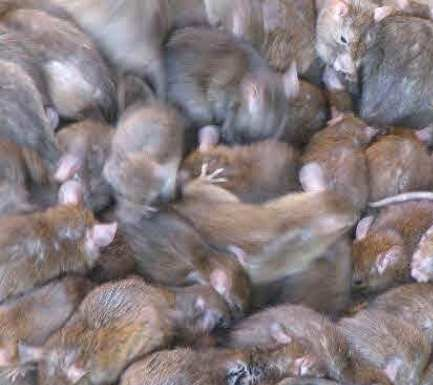
\includegraphics[scale=0.65]{scp/027.jpg}
\linebreak Image taken during initial containment of SCP-027. Subject 027-01 was discovered underneath this pile of rats.
\end{center}
\end{figure}

\textbf{Special Containment Procedures:} The host of SCP-027 (currently subject 027-02) is to be kept in a 5 m x 5 m containment cell with a grated, raised floor connected to a strong vacuum system. All creatures removed from the Subject's containment cell are to be incinerated, except for a small portion to be diverted for analysis and necropsy. The cell is to be cleaned and inspected for structural damage daily.

Subject 027-02 must be monitored by at least two personnel at all times. Any unusual behavior or vital signs on the part of the subject or the appearance of any unusual species in the subject’s vicinity must immediately be reported to Level 4 personnel.

Security personnel assigned to SCP-027 must be inoculated against all known animal-borne pathogens and must be armed with tranquilizer guns, with standing orders to subdue the subject if the need arises.

Until SCP-027 is better understood, no personnel of Level 4 Clearance or higher should approach within 200 m of the Subject.

\textbf{Description:} SCP-027 appears to be a phenomenon of unknown source that seems to be tied to one human subject (currently 027-02) at a time. As host to SCP-027, subject 027-02 is constantly surrounded by swarming vermin that are drawn to his location. The subject does not appear able to assert control over these creatures in any way, and is in fact prone to occasional attacks from feral specimens. These creatures have also been known to attack personnel who approach too closely.

Wherever the subject goes, an initial swarm of flying insects such as gnats and flies will start to form a cloud around him, usually within two to three minutes. Shortly thereafter, crawling animals (including lice, cockroaches, worms, spiders, [DATA EXPUNGED], mice, and rats) will begin to appear; the longer the subject remains in a location, the more vermin will gather there. When the subject leaves a location, some of these creatures will follow, but most will disperse.

SCP-027 has been known to transfer between hosts once, upon the death of the first known host, Subject 027-01 (see Appendix 1 for more information). Since SCP-027 could likely repeat this feat upon the death of Subject 027-02, all high-value personnel should be kept far away from the current host until more about SCP-027 is understood. SCP-027 has also likely transferred between hosts an unknown number of times before containment. Research into potential previous hosts has commenced, with preliminary evidence suggesting that SCP-027 may have existed for at least \censor{XXX} years.

It is not yet known how SCP-027 chooses or attracts animals, or even what SCP-027 exactly is. The previous host never expressed having any sort of communication with a separate conscious entity; analysis of the current host has been inconclusive at best.

---

\textbf{Appendix 1:} Timeline of Significant Events

04/\censor{XX}/199\censor{X}: Subject 027-01 is discovered in an abandoned warehouse outside \censor{XXXXXXX}, \censor{XX}, that had been completely overrun by rats, cockroaches, and other vermin, and is contained and cataloged as SCP-027. The subject is described as a Caucasian male in his late thirties, of average height but gaunt, filthy, and covered in bites and scratches. The subject also shows symptoms of degraded mental health, evidence of heavy use of alcohol and illicit drugs, and signs of prolonged sleep deprivation.

10/\censor{XX}/200\censor{X}: Subject expires. Autopsy shows more than 70\% of the subject’s body \expunged \ a colony of rats nesting in the subject’s abdomen for at least \censor{XX} generations.

10/\censor{XX}/200\censor{X}: Between 140 and 150 hours after the Subject’s death, Security Officer K\censor{XXXXXX} F\censor{XXXXX} reports being awoken by breathing problems due to a large housefly having crawled up his nose (later shown to have lain eggs). Subsequent observations lead to categorization of Officer F\censor{XXXXX} as subject 027-02, the original host is reclassified as subject 027-01, and SCP-027 is redefined.

\expunged

---

\textbf{Appendix 2:} Transcript of Interview 027-201

The following interview was conducted on 10/\censor{XX}/200\censor{X}, shortly after Subject 027-02 was identified and transferred to the containment cell that had housed Subject 027-01.
\begin{leftbar}
\textbf{Dr. Jameson:} Good morning, Officer F\censor{XXXXX}. How are you feeling?

\textbf{Subject 027-02:} Scared. Confused. Mostly scared though.

\textbf{J:} Understandable....

\textbf{S:} And itchy. I feel like I need to shower all the damn time.

\textbf{J:} Ah. But what about, um, inside? Do you feel anything different inside you, like a... presence?

\textbf{S:} \lb thinks, scratches his head\rb \ No, I don't think I do. I haven't really noticed anything like that.

\textbf{J:} You haven't felt anything different since the original host died, besides the itching?

\textbf{S:} No, I can't say I have.

\textbf{J:} What about any sort of voices, or compulsions—

\textbf{S:} \lb agitated\rb \ No, I haven't felt anything except bugs crawling all over me! I feel dirty, and scared, and... Doc, what about my family? You gotta get this thing out of me so I can see them again!

\textbf{J:} Of... of course. We're going to do everything we can to get 027 out of you. God, I... I'm sorry, K\censor{XXXXXX}....
\end{leftbar}

\textbf{Note:} Shortly after this interview took place, Dr. Jameson and several other members of the research team for SCP-027 were transferred to other projects.